% Sandia National Laboratories is a multimission laboratory managed and
% operated by National Technology & Engineering Solutions of Sandia, LLC, a
% wholly owned subsidiary of Honeywell International Inc., for the U.S.
% Department of Energy’s National Nuclear Security Administration under
% contract DE-NA0003525.

% Copyright 2002-2021 National Technology & Engineering Solutions of Sandia,
% LLC (NTESS).

% -------------------------------------------------------------------------
% Sampling Analysis Section ---------------------------------------------------
% -------------------------------------------------------------------------

\clearpage
\section{Polynomial Chaos Expansion methods}
\label{PCE_Analysis}
\label{pce_Overview}
\index{analysis!PCE} \index{PCE analysis} 
\index{\texttt{.SAMPLING}}

\Xyce{} supports several styles of Polynomial Chaos expansion (PCE) methods, which are 
stochastic expansion methods that approximate the functional dependence
of a simulation response on uncertain model parameters by expansion
in a polynomial basis~\cite{XiuKarn02,Xiu2010}.   
In \Xyce{} the Stokhos library~\cite{stokhos} has been used to implement 
generalized PCE methods using the Wiener-Askey scheme\cite{XiuKarn02}.   

To propagate input uncertainty through a model using PCE, \Xyce{}
performs the following steps: (1) input uncertainties are transformed
to a set of uncorrelated random variables, (2) a basis such
as Hermite polynomials is selected, and (3) the parameters of the
functional approximation are determined.  The general PCE 
for a response $O$ has the form:
\begin{equation}
  O(p) \approx \hat{O}(p) = \sum_{i=0}^{P} \alpha^i \varPsi^i(p),
  \label{eq:genPCEresponse}
\end{equation}
where each multivariate basis polynomial $\varPsi^i(p)$ involves products of univariate
polynomials that are tailored to the individual random variables. 
More details about these methods and their \Xyce{} implementation can be found in
reference~\cite{xyceAdvancedUQ} and the references therein.

\Xyce{} supports three versions of polynomial chaos.  They mainly differ in how the coefficients $\alpha$ in equation~\ref{eq:genPCEresponse} are computed.  These three methods are:
\begin{itemize}
  \item Non-intrusive regression polynomial chaos
  \item Non-intrusive spectral projection  (NISP)
  \item Fully intrusive spectral projection
\end{itemize}
The first two versions are non-intrusive, meaning that they don't directly modify the forward problem being solved.  
Instead, they are augmentations to the \texttt{.SAMPLING} and \texttt{.EMBEDDEDSAMPLING} analysis methods.
The fully intrusive method is a separate analysis type, and is invoked using the \texttt{.PCE} command.

\subsection{Regression-based Polynomial Chaos}
\label{regressionPCE}

Regression-based PCE is briefly described here.
Regression-based PCE approaches aim to solve the linear system:
\begin{equation}
\boldsymbol{\varPsi} \boldsymbol{\alpha} \approx \boldsymbol{R} \label{eq:regression}
\end{equation}
for a set of PCE coefficients $\boldsymbol{\alpha}$ that best
reproduce a set of response values $\boldsymbol{R}$.  
The regression approach finds a set of PCE coefficients $\alpha^i$ which best fit a set of response
values obtained from a sampling study on the density function of the uncertain 
parameters~\cite{pt_colloc1}.  One advantage of regression-based methods is that
they are very flexible with respect to the exact sample points used to evaluate the responses, 
and can readily be used with standard sampling methods such as Monte Carlo and Latin Hypercube Sampling.
For this project, the method for solving 
Eq. \eqref{eq:regression} that has been implemented in \Xyce{} is 
least squares regression.

Regression-based PCE can be applied as a post-process step 
to \texttt{.SAMPLING} and \texttt{.EMBEDDEDSAMPLING}.  It is invoked by adding 
\texttt{regression\_pce=true} to the \texttt{.options SAMPLES} 
or \texttt{.options EMBEDDEDSAMPLES} command lines.  

Regression PCE will use the samples selected by the sampling algorithm (Monte Carlo or Latin Hypercube).  
The regression PCE algorithm will \emph{not} estimate the optimal number of samples to use, and so this must 
be set by the user.   For regression PCE, the number of samples needed for an accurate answer
should be smaller than the number that would have been required by conventional sampling.
For regression problems, to get an accurate answer it is considered good practice to oversample 
the basis size by at least a factor of 2. 

A simple example netlist, which uses regression PCE with \texttt{.SAMPLING} is given in figure~\ref{regressionPCE_Netlist1}.  
Results from this calculation, which are sent to terminal output are given in figure~\ref{regressionPCE_Result1}.

\begin{figure}[htbp]
\fontsize{9pt}{10pt}
\begin{centering}
\shadowbox{
\begin{minipage}{0.8\textwidth}
\begin{vquote}
\color{blue}Regression PCE example \color{black}
.param testNorm=\{\color{red}aunif(2k,1k)\color{black}\}
.param R1value=\{testNorm*2.0\}
R2 1 0 6K
R1 1 2 \{R1value\}
v1 2 0 1000V

.dc v1 1000 1000 1
.print dc format=tecplot v(1)
*
\color{red}.SAMPLING useExpr=true

.options SAMPLES numsamples=12
+ regression\_pce=true
+ order=5
+ outputs=\{v(1)\}
+ sample\_type=lhs
+ stdoutput=true
+ resample=true\color{black}
.end
\end{vquote}
\end{minipage}
}
\caption{Voltage divider regression PCE netlist.  The sampling-related commands are in \color{red}red\color{black}.
\label{regressionPCE_Netlist1}}
\end{centering}
\end{figure}

\begin{figure}[htbp]
\fontsize{9pt}{10pt}
\begin{centering}
\shadowbox{
\begin{minipage}{0.8\textwidth}
\begin{vquote}
***** Beginning Latin Hypercube Sampling simulation....

***** Regression PCE enabled.  Number of sample points = 12

***** PCE Basis size = 6

Seeding random number generator with 2412823737

LHS sampling mean of {V(1)} = 614.666
LHS sampling stddev of {V(1)} = 71.4563
LHS sampling variance of {V(1)} = 5106
LHS sampling skew of {V(1)} = 0.299928
LHS sampling kurtosis of {V(1)} = 2.07869
LHS sampling max of {V(1)} = 733.936
LHS sampling min of {V(1)} = 503.315

(traditional sampling) regression PCE mean of {V(1)} = 608.197
(traditional sampling) regression PCE stddev of {V(1)} = 71.3831

Statistics from re-sampling regression PCE approximation of {V(1)}:
mean     = 608.071
stddev   = 70.8532
variance = 5020.18
skew     = 0.298245
kurtosis = 1.93151
max      = 749.652
min      = 500.054
\end{vquote}
\end{minipage}
}
\caption{Voltage divider regression PCE result.
\label{regressionPCE_Result1}}
\end{centering}
\end{figure}

\clearpage
\subsection{Non-Intrusive Spectral Projection (NISP)}
\label{nisp}

The spectral projection PCE approach projects the response
against each basis function $\Psi_j(p)$ using inner
products and employs the polynomial orthogonality properties to
extract each coefficient. Each inner product involves a
multidimensional integral over the support range of the weighting
function, which can be evaluated numerically using sampling,
tensor-product quadrature, Smolyak sparse grid \cite{Smolyak_63}, or
cubature \cite{stroud} approaches.   For the \Xyce{} implementation 
this means evaluating the following equation for each coefficient using 
quadrature rules:
\begin{equation}
\alpha^{i} = \frac{\langle O\varPsi ^{i}\rangle} {\langle (\varPsi ^{i})^{2}\rangle} = \frac{1} {\langle (\varPsi^{i})^{2}\rangle}\int _{\varGamma}O(p ;y)\varPsi ^{i}(y)\rho (y)dy = 0,\quad i = 0,\ldots,P.
  \label{nispProjection}
\end{equation}
In this equation $\rho$ is the joint density function, with respect to which the polynomials $\varPsi^i$ are orthogonal.
Evaluating this equation requires solving the integral on the right hand side.  
While many methods for solving this integral could be used, for the NISP algorithm 
the integral is solved using Gaussian Quadrature and related methods.  For this 
reason, these methods are sometimes referred to as ``quadrature PCE'' methods.
Stokhos supports several quadrature methods, and supplies the necessary quadrature points 
to \Xyce{} for the specified details.  

To solve the integral using quadrature, \Xyce{} has to evaluate the forward problem at 
the various quadrature points. In this reguard, this is similar to the
regression methods described in section~\ref{regressionPCE}, which has to do 
forward evaluations at randomly sampled points.
Since NISP uses quadrature points, the points are completely deterministic, 
and there are no random numbers involved.
The number of quadrature points can increase exponentially for larger numbers of uncertain 
parameters, but this can be mitigated by using sparse grid techniques.  

Non-intrusive spectral projection PCE can be applied as a post-process step 
to \texttt{.SAMPLING} and \texttt{.EMBEDDEDSAMPLING}.  It is invoked by adding 
\texttt{projection\_pce=true} to the \texttt{.options SAMPLES} 
or \texttt{.options EMBEDDEDSAMPLES} command lines.

As noted, when using NISP it is not necessary to specify the number of sample points, as they will
be set by the quadrature algorithm.  To enable quadrature on a sparse grid, set the 
option \texttt{sparse\_grid=true} on the \texttt{.options EMBEDDEDSAMPLES} command line.

\subsection{Fully Intrusive Spectral Projection}
\label{intrusivePCE}
The fully intrusive form of PCE involves solving a system of equations which is constructed by 
applying the orthogonal polynomial expansion defined by 
Eq. \eqref{eq:genPCEresponse} to all the terms of the differential-algebraic 
system of equations solved by \Xyce{}.  The details of this construction are given in 
reference~\cite{xyceAdvancedUQ}.

\clearpage
%% -----------------------------------------------------------------------------------
\subsection{Gilbert Cell Mixer PCE example}
\label{xyceGilbertCell}
A Gilbert cell mixer circuit is given in figure~\ref{gilbert}~\cite{1049925}.  A corresponding netlist 
is given in Fig.~\ref{NISP_gilbert_netlist}.
In this circuit, the LO voltage is given by \texttt{v(6,2)} and \texttt{v(15,10)} is the input. 
The output is the difference between collector voltages of Q4/Q6 and Q3/Q5 (\texttt{V(5,3)}), 
and should be the approximate product of the LO and input voltages.
\begin{figure}[hbt]
\centering
\resizebox{.9\linewidth}{!}{ \input cktFigs/gilbert}
  \caption[Gilbert cell mixer schematic]
  {Gilbert cell mixer schematic.}
\label{gilbert}
\end{figure}
In this example, all eight 
resistors are given uncertain resistances, distributed with the following normal distributions:  R1 and R2 are N(10,1), 
R5 and R6 are N(100,5), and R3, R4, R7, and R8 are N(1500,50).  These large standard deviations of the resistances are 
not realistic, but are chosen for demonstration purposes.

Ensemble and PCE results for the Gilbert cell mixer are shown in figure~\ref{gilbert_compare}.   
As this calculation was concerned with the transient behavior, only \texttt{.EMBEDDEDSAMPLING} 
and \texttt{.PCE} are used in this example.  For \texttt{.EMBEDDEDSAMPLING}, both types of 
non-intrusive PCE are used.
The light grey lines in Fig.~\ref{gilbert_compare} are for all the sample points 
of an embedded LHS study with 1000 samples.    The red lines (which are obscured 
by other results) show the mean and the mean +/- twice the standard deviation for the 
1000 sample study.  This can be considered the ``gold'' standard for this simulation.
The other solid lines show the moments from the various PCE calculations, and they 
lie on top of the 1000 LHS sample moments.  

This version of the netlistgiven in Fig.~\ref{NISP_gilbert_netlist}
is using non-intrusive projection PCE as an augmentation to \texttt{.EMBEDDEDSAMPLING}.  
To convert this netlist to 
use the fully intrusive method, change \texttt{.EMBEDDEDSAMPLING} to \texttt{.PCE}, and 
change \texttt{.options EMBEDDEDSAMPLES} to \texttt{.options PCES}.   Otherwise, the commands are completely the same.
As the number of uncertain parameters is a little bit larger (8), for the projection-based methods a 
Smolyak sparse grid~\cite{Smolyak_63} method is used.  This is set with the  \texttt{sparse\_grid=true} parameter. 
Using the sparse grid, the number of 
required quadrature points for this problem is 129.  Using the non-sparse Gaussian quadrature 
would have required 6561 quadrature points. This would have rendered the method much 
less efficient than sampling, and basically not usable, especially for the \texttt{.PCE} method.

To change the netlist to use non-intrusive regression PCE, change \texttt{projection\_pce=true} 
to \texttt{regression\_pce=true}.  Delete the \texttt{sparse\_grid=true} parameter, as 
it isn't relevant to regression PCE.  

As noted, for regression PCE the number of parameters needs to be set.  Unlike projection-based methods, 
regression PCE does not have a rigid requirement for the number of samples.  For this 
problem the size of the polynomial basis is 45, and for regression problems it 
is considered good practice to oversample by at least a factor of 2, which implies that
a good choice for this circuit is 90 sample points.   
To set this, add \texttt{numsamples=90} on the \texttt{.options EMBEDDEDSAMPLES} line.  
It appears that 90 sampling points was 
adequate for the regression form of PCE, as the all the statistical moments 
match well throughout the transient.

\begin{figure}[htbp]
\fontsize{10pt}{11pt}
\begin{centering}
\shadowbox{
\begin{minipage}{0.95\textwidth}
  \begin{vquote}\color{blue}
* Gilbert cell mixer\color{black}
R5 1 2 \color{red}\{agauss(100,5,1)\}\color{black}
Q3 3 2 4 QB2T2222
Q4 5 6 4 QB2T2222
Q5 3 6 8 QB2T2222
Q6 5 2 8 QB2T2222
R6 2 1 \color{red}\{agauss(100,5,1)\}\color{black}
*the local oscillator
VLO 6 2 DC 0 SIN(0 .05V 4e7 0 0)
Q1 4 10 11 QB2T2222
R1 11 12 \color{red}\{agauss(10,1,1)\}\color{black}
R2 12 13 \color{red}\{agauss(10,1,1)\}\color{black}
* input bias current
I1 12 0 DC 1.8mA
Q2 8 15 13 QB2T2222
R4 15 16 \color{red}\{agauss(1500,50,1)\}\color{black}
R3 16 10 \color{red}\{agauss(1500,50,1)\}\color{black}
V1 16 0 DC 1.8V
*the input voltage to be mixed with the LO
V5 15 10 DC 0 sin(0 .05V 3e6 0 0)
R7 5 17 \color{red}\{agauss(1500,50,1)\}\color{black}
R8 3 17 \color{red}\{agauss(1500,50,1)\}\color{black}
V3 17 0 DC 8V
V2 1 0 DC 6V

.MODEL QB2T2222  NPN (
+ IS=3.136905E-14 BF=189 NF=0.9977664 VAF=29.7280913
+ IKF=0.7405619 ISE=8.49314E-15 NE=1.3186316 BR=38.9531224
+ NR=0.9833179 VAR=28.5119855 IKR=4.632395E-3 ISC=4.624043E-14
+ NC=1.225899 RB=2.0158781 IRB=0.0227681 RBM=0.9730261
+ RE=0.0501513 RC=0.6333 CJE=2.369655E-11 VJE=0.6884357
+ MJE=0.3054743 TF=5.3E-10 XTF=48.5321578 VTF=5.3020062
+ ITF=1.1 PTF=14.6099207 CJC=8.602583E-12 VJC=0.4708887
+ MJC=0.3063885 XCJC=1 TR=74E-9 CJS=1e-12 VJS=.75
+ MJS=0 XTB=0.87435 EG=1.11 XTI=5.825
+ KF=0 AF=1 FC=0.5)

.TRAN 1ns 3e-7
.PRINT TRAN format=tecplot v(6,2) v(15,10) v(5,3)
.options timeint reltol=1.0e-5 
    \color{red}
.EMBEDDEDSAMPLING useExpr=true
.options EMBEDDEDSAMPLES projection\_pce=true 
+ outputs={v(5,3)} order=2 sparse\_grid=true \color{black}
.end
\color{blue}\end{vquote}
\end{minipage}
}
\caption{Gilbert Cell Non-Instrusive Spectral Project (NISP) netlist.  
  UQ commands are in \color{red}red\color{black}, and NISP is specified using the \texttt{projection\_pce} parameter.
\label{NISP_gilbert_netlist}}
\end{centering}
\end{figure}

NISP is used in conjunction with embedded sampling, 
and as noted requires 129 sample points if using sparse grid quadrature.  Fully 
intrusive PCE, which uses all the same machinery as NISP also requires 129 
quadrature points.  



\begin{figure}[hbt]
\centering
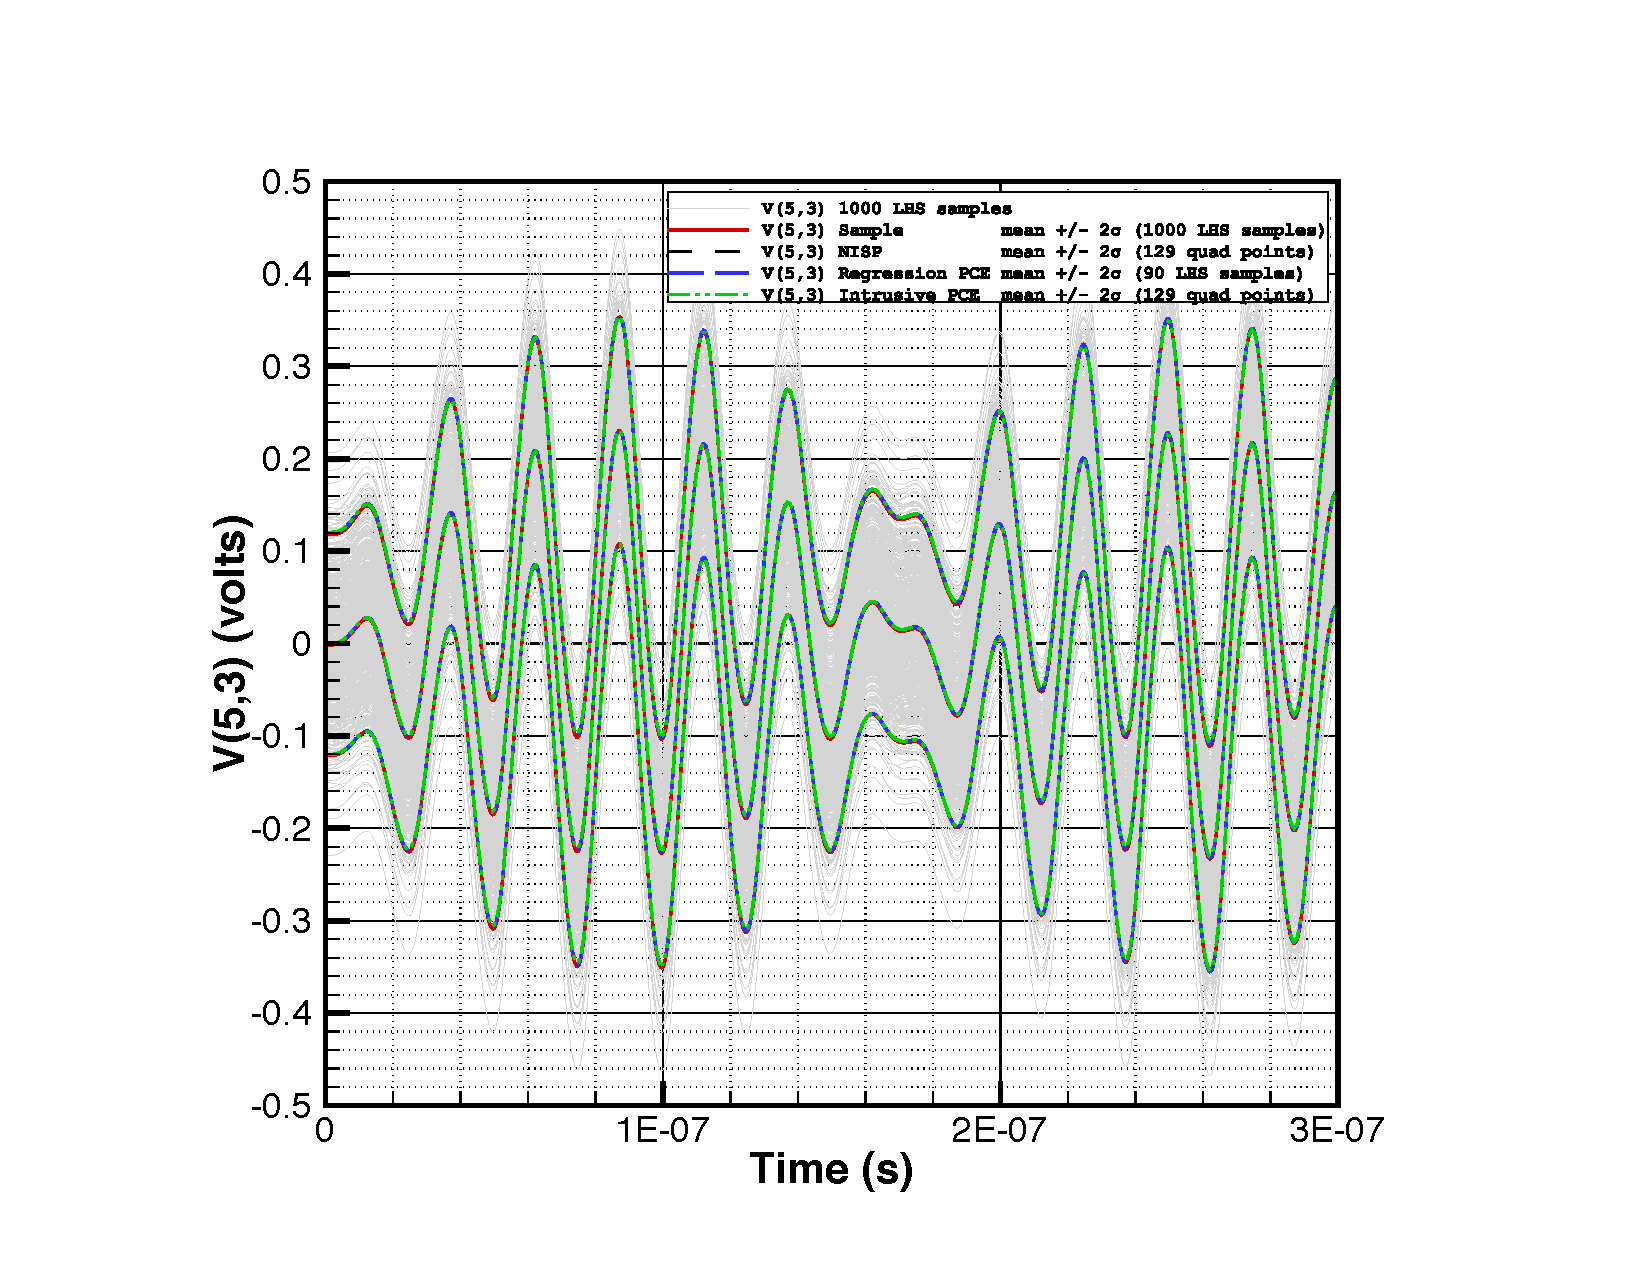
\includegraphics[width=5in]{gilbert_compare2.pdf}
\caption
  [Gilbert Cell Mixer Output for several \Xyce{} embedded UQ methods]
  {Gilbert Cell Mixer Output for several \Xyce{} embedded UQ methods.  The mean and standard deviations for all the methods (Embedded LHS sampling, NISP, Regression PCE and fully intrusive PCE) all match very well.}
\label{gilbert_compare}
\end{figure}

\clearpage
